\begin{flushright} {\tiny {\color{gray} q1q13D\_2bubbles.tex}} \end{flushright}

This element is implemented in \stone 82.
The two bubble functions are given in Karabelas \etal (2020) \cite{kahp20}:
\begin{eqnarray}
b_9(r,s,t) &=& \left(\frac{27}{32}\right)^3 (1-r^2)(1-s^2)(1-t^2) \cdot (1-r)(1-s)(1-t) 
= \beta_9(r)\cdot\beta_9(s) \cdot \beta_9(t) \\
b_{10}(r,s,t) &=& \left(\frac{27}{32}\right)^3 (1-r^2)(1-s^2)(1-t^2) \cdot (1+r)(1+s)(1+t) 
= \beta_{10}(r)\cdot\beta_{10}(s) \cdot \beta_{10}(t) 
\end{eqnarray}
where I have chosen nodes 1 ($\vec{r}_1=(-1,-1,-1)$) and 7 ($\vec{r}_7=(+1,+1,+1)$) 
as diagonally opposed nodes (a requirement from the paper), 
and with
\[
\beta_9(x)=\frac{27}{32} (1-x^2) (1-x)
\qquad
\beta_{10}(x)=\frac{27}{32} (1-x^2) (1+x)
\]

I have added the $(27/32)^3$ coefficients so that these functions are exactly 1 a their 
corresponding nodes.
The term $(1-r^2)(1-s^2)(1-t^2)$ makes sure that the two bubbles are conforming and exactly zero 
on the 6 faces of the element.
In what follows $\tilde{\bN}_{1..8}$ are the standard $Q_1$ basis functions.

\begin{center}
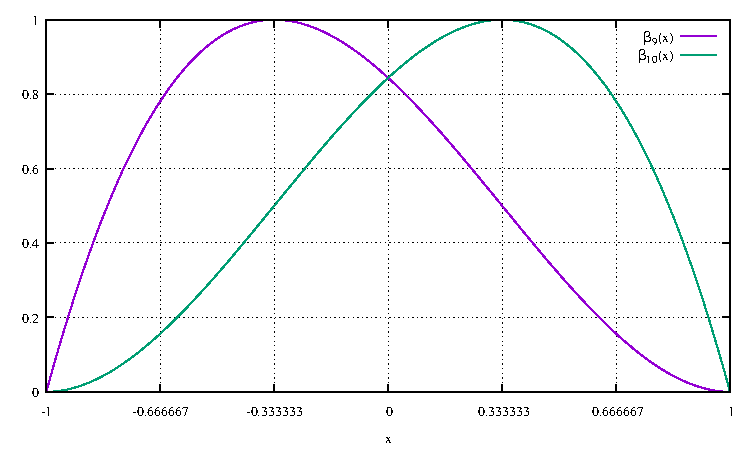
\includegraphics[width=8cm]{images/MINI3D/bubbles.pdf}\\
{\captionfont Representation of bubbles $\beta_9(x)$ and $\beta_{10}(x)$}
\end{center}

\begin{remark}
Bubble function 9 is not zero at node 10 and vice versa!
\end{remark}

The authors state: "This also allows for a straightforward inclusion in combination 
with existing finite element codes since all required
implementations are purely on the element level". This is especially true 
if static condensation is used (the authors explain static condensation 
for the bubbles in the appendix of the paper).

The ten nodes are the standard 8 corners of the $Q_1$ element as well  
as $\vec{r}_9=(-1/3,-1/3,-1/3)$ for $b_9$ and 
$\vec{r}_{10}=(1/3,1/3,1/3)$ for $b_{10}$.
We have the following approximation of function $f$ inside the element:
\[
f^h(r,s,t) = \sum_{i=1}^{8} a_i \tilde{\bN}_i(r,s,t) + a_9 b_9(r,s,t) + a_{10} b_{10}(r,s,t)
\]
We notice that bubble functions are exactly zero at the corners of the reference element and
we can compute the values of the ten polynomials ($\tilde{N}_{1-8}(r,s,t),b_9(r,s,t),b_{10}(r,s,t)$) 
at the ten nodes:
\[
\begin{array}{c|cccccccccc}
 & \tilde{\bN}_1 & \tilde{\bN}_2 & \tilde{\bN}_3 & \tilde{\bN}_4 & \tilde{\bN}_5 
 & \tilde{\bN}_6 & \tilde{\bN}_7 & \tilde{\bN}_8 & b_9 & b_{10}\\
 \hline\hline
\vec{r}_1=(-1,-1,-1)    &1 &0 &0 &0 &0 &0 &0 &0 &0 &0 \\
\vec{r}_2=(+1,-1,-1)    &0 &1 &0 &0 &0 &0 &0 &0 &0 &0 \\
\vec{r}_3=(+1,+1,-1)    &0 &0 &1 &0 &0 &0 &0 &0 &0 &0 \\
\vec{r}_4=(-1,+1,-1)    &0 &0 &0 &1 &0 &0 &0 &0 &0 &0 \\
\vec{r}_5=(-1,-1,+1)    &0 &0 &0 &0 &1 &0 &0 &0 &0 &0 \\
\vec{r}_6=(+1,-1,+1)    &0 &0 &0 &0 &0 &1 &0 &0 &0 &0 \\
\vec{r}_7=(+1,+1,+1)    &0 &0 &0 &0 &0 &0 &1 &0 &0 &0 \\
\vec{r}_8=(-1,+1,+1)    &0 &0 &0 &0 &0 &0 &0 &1 &0 &0 \\
\vec{r}_9=(-\frac13,-\frac13,-\frac13)    &8/27 & 4/27 & 2/27  & 4/27 & 4/27 & 2/27& 1/27& 2/27 &1 & 1/8\\
\vec{r}_{10}=(+\frac13,+\frac13,+\frac13) &1/27 & 2/17 & 4/27 & 2/27 & 2/27& 4/27& 8/27& 4/27& 1/8  &1 \\
\end{array}
\]




We then require that the polynomial representation of $f^h$ of $f$ inside the element
is such that $f^h(\vec{r}_i)=f_i$, i.e.:
\begin{eqnarray}
f_1 = f^h(r_1,s_1,t_1) &=& a_1  \nonumber\\
f_2 = f^h(r_2,s_1,t_1) &=& a_2  \nonumber\\
f_3 = f^h(r_3,s_1,t_1) &=& a_3  \nonumber\\
f_4 = f^h(r_4,s_1,t_1) &=& a_4  \nonumber\\
f_5 = f^h(r_5,s_1,t_1) &=& a_5  \nonumber\\
f_6 = f^h(r_6,s_1,t_1) &=& a_6  \nonumber\\
f_7 = f^h(r_7,s_1,t_1) &=& a_7  \nonumber\\
f_8 = f^h(r_8,s_1,t_1) &=& a_8  \nonumber\\
f_9 = f^h(r_9,s_9,t_9) &=&  \frac{1}{27} (8a_1 + 4a_2 + 2a_3 +4a_4 + 4a_5 + 2a_6 + a_7 +2a_8)  + a_9 + a_{10}/8 
\nonumber\\
f_{10} = f^h(r_{10},s_{10},t_{10}) &=& \frac{1}{27} (a_1 + 2a_2 + 4a_3 +2a_4 + 2a_5 + 4a_6 + 8a_7 +4a_8)  + a_9/8 + a_{10} \nonumber
\end{eqnarray}
or,
\[
\left(
\begin{array}{cccccccccc}
1 &0 &0 &0 &0 &0 &0 &0 &0 &0 \\
0 &1 &0 &0 &0 &0 &0 &0 &0 &0 \\
0 &0 &1 &0 &0 &0 &0 &0 &0 &0 \\
0 &0 &0 &1 &0 &0 &0 &0 &0 &0 \\
0 &0 &0 &0 &1 &0 &0 &0 &0 &0 \\
0 &0 &0 &0 &0 &1 &0 &0 &0 &0 \\
0 &0 &0 &0 &0 &0 &1 &0 &0 &0 \\
0 &0 &0 &0 &0 &0 &0 &1 &0 &0 \\
8/27 & 4/27 & 2/27  & 4/27 & 4/27 & 2/27& 1/27& 2/27 &1 & 1/8\\
1/27 & 2/17 & 4/27 & 2/27 & 2/27& 4/27& 8/27& 4/27& 1/8  &1 
\end{array}
\right)
\cdot
\left(
\begin{array}{c}
a_1 \\ a_2 \\ a_3 \\ a_4 \\ a_5 \\ a_6 \\ a_7 \\ a_8 \\ a_9 \\ a_{10}
\end{array}
\right)
=
\left(
\begin{array}{c}
f_1 \\ f_2 \\ f_3 \\ f_4 \\ f_5 \\ f_6 \\ f_7 \\ f_8 \\ f_9 \\ f_{10}
\end{array}
\right)
\]
which yields $a_i=f_i$ for $i=1,...8$ and 
\begin{eqnarray}
a_9 + a_{10}/8 &=& f_9\underbrace{-\frac{1}{27} (8f_1 + 4f_2 + 2f_3 +4f_4 + 4f_5 + 2f_6 + f_7 +2f_8)}_{\tilde{f}_9}   
\nonumber\\
a_9/8 + a_{10} &=& f_{10}
\underbrace{-\frac{1}{27} (f_1 + 2f_2 + 4f_3 +2f_4 + 2f_5 + 4f_6 + 8f_7 +4f_8)}_{\tilde{f}_{10}} 
\nonumber
\end{eqnarray}

\begin{eqnarray}
8a_9 + a_{10} &=& 8f_9 + 8\tilde{f}_9  \nonumber\\
a_9 + 8a_{10} &=& 8f_{10} +8\tilde{f}_{10}
\nonumber
\end{eqnarray}
and then 
\begin{eqnarray}
a_{9}
&=&\frac{1}{63}(64 {f}_{9}-8{f}_{10}) + \frac{1}{63}(64 \tilde{f}_{9}-8\tilde{f}_{10}) \nonumber\\
&=& \frac{8}{63}(8{f}_{9}-{f}_{10})+\frac{8}{63}(8\tilde{f}_{9}-\tilde{f}_{10}) \nonumber\\
&=& \frac{8}{63}(8{f}_{9}-{f}_{10}) -\frac{1}{27}\frac{8}{63}
\left[ 8 (8f_1 + 4f_2 + 2f_3 +4f_4 + 4f_5 + 2f_6 + f_7 +2f_8) \right. \nonumber\\
&& \left. - (f_1 + 2f_2 + 4f_3 +2f_4 + 2f_5 + 4f_6 + 8f_7 +4f_8) \right] \nonumber\\
&=& \frac{8}{63}(8{f}_{9}-{f}_{10}) -\frac{1}{27}\frac{8}{63} 
( 63 f_1 +30 f_2 +12 f_3  +30f_4 +30f_5 +12f_6 +12f_8)\nonumber\\ \nonumber \\
a_{10} 
&=& \frac{1}{63}(64 {f}_{10}-8{f}_9) + \frac{1}{63}(64 \tilde{f}_{10}-8\tilde{f}_9) \nonumber\\
&=& \frac{8}{63}(8 {f}_{10}-{f}_9) + \frac{8}{63}(8 \tilde{f}_{10}-\tilde{f}_9) \nonumber\\
&=& \frac{8}{63}(8 {f}_{10}-{f}_9) -\frac{1}{27}\frac{8}{63} \left[
8(f_1 + 2f_2 + 4f_3 +2f_4 + 2f_5 + 4f_6 + 8f_7 +4f_8) \right. \nonumber\\
&& \left. -(8f_1 + 4f_2 + 2f_3 +4f_4 + 4f_5 + 2f_6 + f_7 +2f_8)
\right] \nonumber\\
&=&\frac{8}{63}(8 {f}_{10}-{f}_9) -\frac{1}{27}\frac{8}{63} 
(12f_2 + 30f_3 + 12f_4 +12f_5 + 30f_6 + 63f_7 +30f_8      ) \nonumber
\end{eqnarray}

We can then write

\begin{eqnarray}
f^h(r,s,t) 
&=& f_1 \bN_1(r,s,t) + f_2 \bN_2(r,s,t) + f_3 \bN_3(r,s,t) + f_4 \bN_4(r,s,t) \nonumber\\
&+& f_5 \bN_5(r,s,t) + f_6 \bN_6(r,s,t) + f_7 \bN_7(r,s,t) + f_8 \bN_8(r,s,t) \nonumber\\
&+& \left[\frac{8}{63}(8{f}_{9}-{f}_{10})-\frac{1}{27}\frac{8}{63}  ( 63 f_1 +30 f_2 +12 f_3  +30f_4 +30f_5 +12f_6 +12f_8) \right] b_9(r,s,t) \nonumber\\
&&\left[ \frac{8}{63}(8 {f}_{10}-{f}_9)  -\frac{1}{27}\frac{8}{63} (12f_2 + 30f_3 + 12f_4 +12f_5 + 30f_6 + 63f_7 +30f_8) \right] b_{10}(r,s,t) \nonumber\\
%&=& \left(N_1(r,s,t) - \frac{8}{27}b_9(r,s,t) \right) f_1 \nonumber\\
%&+& \left(N_2(r,s,t) - \frac{30}{27}\frac{8}{63} b_9(r,s,t) - \frac{12}{27}\frac{8}{63} b_{10}(r,s,t)  \right) f_2 \nonumber\\
%&+&\left( N_3(r,s,t)  -\frac{12}{27}\frac{8}{63} b_9r,s,t) -\frac{30}{27}\frac{8}{63} b_{10}(r,s,t)  \right)f_3 \nonumber\\
%&+& \left( N_4(r,s,t) -\frac{30}{27}\frac{8}{63} b_{9}r,s,t) -\frac{12}{27}\frac{8}{63} b_{10}r,s,t)\right)f_4 \nonumber\\ 
%&+&\left( N_5(r,s,t)- \frac{30}{27}\frac{8}{63} b_{9}r,s,t) -\frac{12}{27}\frac{8}{63} b_{10}r,s,t) \right) f_5 \nonumber\\
%&+&\left( N_6(r,s,t) -\frac{12}{27}\frac{8}{63} b_9r,s,t) -\frac{30}{27}\frac{8}{63} b_{10}r,s,t) \right) f_6 \nonumber\\
%&+&\left( N_7(r,s,t) - \frac{8}{27}b_{10}(r,s,t) \right) f_7 \nonumber\\
%&+&\left(N_8(r,s,t) -\frac{12}{27}\frac{8}{63} b_9(r,s,t) -\frac{30}{27}\frac{8}{63} b_{10}(r,s,t) \right) f_8 \nonumber\\
%&+& \left(  \frac{64}{63}b_9(r,s,t) -\frac{8}{63} b_{10}(r,s,t) \right) f_9 
%+ \left( -\frac{8}{63} b_{9}(r,s,t)  + \frac{64}{63}b_{10}(r,s,t) \right) f_{10} \nonumber\\
&=& \left(\bN_1(r,s,t) - \frac{2^3}{3^3}b_9(r,s,t) \right) f_1 \nonumber\\
&+& \left(\bN_2(r,s,t) - \frac{2^3}{3^3}\frac{10}{21} b_9(r,s,t) - \frac{2^3}{3^3}\frac{4}{21} b_{10}(r,s,t)  \right) f_2 \nonumber\\
&+&\left( \bN_3(r,s,t)  -\frac{2^3}{3^3}\frac{4}{21} b_9r,s,t) -\frac{2^3}{3^3}\frac{10}{21} b_{10}(r,s,t)  \right)f_3 \nonumber\\
&+& \left( \bN_4(r,s,t) -\frac{2^3}{3^3}\frac{10}{21} b_{9}r,s,t) -\frac{2^3}{3^3}\frac{4}{21} b_{10}(r,s,t)\right)f_4 \nonumber\\ 
&+&\left( \bN_5(r,s,t)- \frac{2^3}{3^3}\frac{10}{21} b_{9}r,s,t) -\frac{2^3}{3^3}\frac{4}{21} b_{10}(r,s,t) \right) f_5 \nonumber\\
&+&\left( \bN_6(r,s,t) -\frac{2^3}{3^3}\frac{4}{21} b_9(r,s,t) -\frac{2^3}{3^3}\frac{10}{21} b_{10}(r,s,t) \right) f_6 \nonumber\\
&+&\left( \bN_7(r,s,t) - \frac{2^3}{3^3}b_{10}(r,s,t) \right) f_7 \nonumber\\
&+&\left( \bN_8(r,s,t) -\frac{2^3}{3^3}\frac{4}{21} b_9(r,s,t) -\frac{2^3}{3^3}\frac{10}{21} b_{10}(r,s,t) \right) f_8 \nonumber\\
&+& \left(  \frac{64}{63}b_9(r,s,t) -\frac{8}{63} b_{10}(r,s,t) \right) f_9 
+ \left( -\frac{8}{63} b_{9}(r,s,t)  + \frac{64}{63}b_{10}(r,s,t) \right) f_{10} 
\end{eqnarray}

and finally arrive at the basis functions:
\begin{mdframed}[backgroundcolor=blue!5]
\begin{eqnarray}
\bN_1(r,s,t)    &=&  \tilde{\bN}_1(r,s,t) - \frac{2^3}{3^3}b_9(r,s,t)      \nonumber\\
\bN_2(r,s,t)    &=&  \tilde{\bN}_2(r,s,t) - \frac{2^3}{3^3}\frac{10}{21} b_9(r,s,t) - \frac{2^3}{3^3}\frac{4}{21} b_{10}(r,s,t)      \nonumber\\
\bN_3(r,s,t)    &=&  \tilde{\bN}_3(r,s,t)  -\frac{2^3}{3^3}\frac{4}{21} b_9(r,s,t) -\frac{2^3}{3^3}\frac{10}{21} b_{10}(r,s,t)      \nonumber\\
\bN_4(r,s,t)    &=&  \tilde{\bN}_4(r,s,t) -\frac{2^3}{3^3}\frac{10}{21} b_{9}(r,s,t) -\frac{2^3}{3^3}\frac{4}{21} b_{10}r,s,t)      \nonumber\\
\bN_5(r,s,t)    &=&  \tilde{\bN}_5(r,s,t)- \frac{2^3}{3^3}\frac{10}{21} b_{9}(r,s,t) -\frac{2^3}{3^3}\frac{4}{21} b_{10}(r,s,t)      \nonumber\\
\bN_6(r,s,t)    &=&  \tilde{\bN}_6(r,s,t) -\frac{2^3}{3^3}\frac{4}{21} b_9(r,s,t) -\frac{2^3}{3^3}\frac{10}{21} b_{10}(r,s,t)      \nonumber\\
\bN_7(r,s,t)    &=&  \tilde{\bN}_7(r,s,t) - \frac{2^3}{3^3}b_{10}(r,s,t)      \nonumber\\
\bN_8(r,s,t)    &=&  \tilde{\bN}_8(r,s,t) -\frac{2^3}{3^3}\frac{4}{21} b_9(r,s,t) -\frac{2^3}{3^3}\frac{10}{21} b_{10}(r,s,t)      \nonumber\\
\bN_9(r,s,t)    &=&  \frac{64}{63}b_9(r,s,t) -\frac{8}{63} b_{10}(r,s,t)      \nonumber\\
\bN_{10}(r,s,t) &=&  -\frac{8}{63} b_{9}(r,s,t)  + \frac{64}{63}b_{10}(r,s,t)       \nonumber
\end{eqnarray}
\end{mdframed}

These are somewhat complex forms for the basis functions so we wish to verify the simple property $\sum \bN_i(r,s,t) =1$ 
for all $(r,s,t)$ inside the element:
\begin{eqnarray}
\sum_{i=1}^{10} \bN_i(r,s,t)  
&=& \sum_{i=1}^{8} \tilde{\bN}_i(r,s,t) \nonumber\\
&+& \left[\frac{2^3}{3^3} \left(-1 -\frac{10}{21} -\frac{4}{21} -\frac{10}{21} -\frac{10}{21} -\frac{4}{21} -\frac{4}{21}\right) + \frac{64}{63} -\frac{8}{63} \right] b_9(r,s,t) \nonumber\\
&+& \left[\frac{2^3}{3^3} \left(-\frac{4}{21} -\frac{10}{21} -\frac{4}{21} -\frac{4}{21} -\frac{10}{21} -1 -\frac{10}{21} \right) -\frac{8}{63} + \frac{64}{63} \right] b_{10}(r,s,t) \nonumber\\
&=& 1 + \left[\frac{2^3}{3^3} (-1 -42/21) +\frac{56}{63}  \right] b_9(r,s,t) 
+ \left[\frac{2^3}{3^3} (-42/21 -1)  + \frac{56}{63} \right] b_{10}(r,s,t) \nonumber\\
&=& 1 + \left[\frac{2^3}{3^3} (-3) + \frac{8}{9} \right] b_9(r,s,t) 
+ \left[\frac{2^3}{3^3} (-3)  + \frac{8}{9} \right] b_{10}(r,s,t) \nonumber\\
&=& 1
\end{eqnarray}
Let us move to first order consistency with $f(r)=r$:
\begin{eqnarray}
f^h(r,s,t)
=\sum_{i=1}^{10} \bN_i(r,s,t) f_i
=\sum_{i=1}^{10} \bN_i(r,s,t) r_i 
\end{eqnarray}
It has been established for the $\tilde{\bN}_i$ functions so we are left with
\begin{eqnarray}
f^h(r,s,t)
&=& \underbrace{\sum_{i=1}^8 \tilde{\bN}_i r_i }_{=r} \nn\\
&& -\frac{2^3}{3^3}b_9(r,s,t) (-1)  \nn\\
&& -\frac{2^3}{3^3}\frac{10}{21} b_9(r,s,t) (+1) - \frac{2^3}{3^3}\frac{4}{21} b_{10}(r,s,t) (+1)  \nn\\
&& -\frac{2^3}{3^3}\frac{4}{21} b_9(r,s,t)  (+1)-\frac{2^3}{3^3}\frac{10}{21} b_{10}(r,s,t) (+1)     \nn\\
&&-\frac{2^3}{3^3}\frac{10}{21} b_{9}(r,s,t) (-1) -\frac{2^3}{3^3}\frac{4}{21} b_{10}r,s,t) (-1)     \nn\\
&&- \frac{2^3}{3^3}\frac{10}{21} b_{9}(r,s,t) (-1) -\frac{2^3}{3^3}\frac{4}{21} b_{10}(r,s,t)  (-1)    \nn\\
&& -\frac{2^3}{3^3}\frac{4}{21} b_9(r,s,t) (+1) -\frac{2^3}{3^3}\frac{10}{21} b_{10}(r,s,t) (+1)  \nn\\
&& - \frac{2^3}{3^3}b_{10}(r,s,t) (+1)     \nonumber\\
&&-\frac{2^3}{3^3}\frac{4}{21} b_9(r,s,t) (-1) -\frac{2^3}{3^3}\frac{10}{21} b_{10}(r,s,t) (-1)      \nonumber\\
&& +  \frac{64}{63}b_9(r,s,t)(-1/3) -\frac{8}{63} b_{10}(r,s,t) (-1/3)     \nn\\
&&  -\frac{8}{63} b_{9}(r,s,t)(+1/3)  + \frac{64}{63}b_{10}(r,s,t)   (+1/3) \nn\\
&=& r + 
b_9(r,s,t) \left( 
\frac{8}{27} -\frac{8}{27}\frac{10}{21} -\frac{8}{27}\frac{4}{21} 
+\frac{8}{27}\frac{10}{21}
+\frac{8}{27}\frac{10}{21} 
-\frac{8}{27}\frac{4}{21}  
+\frac{8}{27}\frac{4}{21}
-\frac{64}{189}-\frac{8}{189}
\right) \nn\\ 
&+& b_{10}(r,s,t) \left(
-\frac{8}{27} \frac{4}{21} 
-\frac{8}{27}\frac{10}{21} 
+ \frac{8}{27}\frac{4}{21} 
+ \frac{8}{27}\frac{4}{21} 
-\frac{8}{27}\frac{10}{21} 
-\frac{8}{27}
+\frac{8}{27}\frac{10}{21}
+\frac{8}{189}
+\frac{64}{189}
\right) \nn\\
&=& r +  
b_9(r,s,t) \frac{8}{27} 
\underbrace{\left( 1 - \frac{10}{21} - \frac{4}{21} + \frac{10}{21} + \frac{10}{21} 
-\frac{9}{7} \right)}_{=0}
+b_{10}(r,s,t) \frac{8}{27} 
\underbrace{\left( 
- \frac{4}{21} -\frac{10}{21} + \frac{4}{21} + \frac{4}{21} - \frac{10}{21} -1 +  \frac{10}{21} + \frac{9}{7}
\right)}_{=0} \nn\\
&=& r 
\end{eqnarray}
which proves first-order consistency.





The derivatives of the $\tilde{\bN}_i$ basis functions are already established so we only focus on the spatial derivatives of the bubble functions:
\begin{eqnarray}
\frac{\partial b_9}{\partial r} 
%&=& \left(\frac{27}{32}\right)^3 (1-s^2)(1-t^2) (1-s)(1-t) 
%\frac{\partial }{\partial r} (1-r-r^2+r^3  ) \nonumber\\
&=& \left(\frac{27}{32}\right)^3 (1-s^2)(1-t^2) (1-s)(1-t) (-1-2r+3r^2  )\nonumber\\
\frac{\partial b_9}{\partial s}
&=& \left(\frac{27}{32}\right)^3 (1-r^2)(1-t^2) (1-r)(1-t) (-1-2s+3s^2  )\nonumber\\
\frac{\partial b_9}{\partial t}
&=& \left(\frac{27}{32}\right)^3 (1-r^2)(1-s^2) (1-r)(1-s) (-1-2t+3t^2  )\nonumber\\
\frac{\partial b_{10}}{\partial r} 
%&=& \left(\frac{27}{32}\right)^3 (1-s^2)(1-t^2) (1+s)(1+t) 
%\frac{\partial }{\partial r} (1+r-r^2-r^3  )\nonumber\\
&=& \left(\frac{27}{32}\right)^3 (1-s^2)(1-t^2) (1+s)(1+t) (1-2r-3r^2  )\nonumber\\
\frac{\partial b_{10}}{\partial s}
&=& \left(\frac{27}{32}\right)^3 (1-r^2)(1-t^2) (1+r)(1+t) (1-2s-3s^2  )\nonumber\\
\frac{\partial b_{10}}{\partial t} 
&=& \left(\frac{27}{32}\right)^3 (1-r^2)(1-s^2) (1+r)(1+s) (1-2t-3t^2  ) \nonumber
\end{eqnarray}



\Literature: \textcite{fofo85} (1985), \textcite{sofo87} (1987)

Bishnu talksabout Nitsche bc ? press error near boundary in fofo85
















